%%%%%%%%%%%%%%%%%%%%%%%%%%%%%%%%%%%%%
%                                   %
% Compile with XeLaTeX and biber    %
%                                   %
% Questions or comments:            %
%                                   %
% joshua dot mcneill at uga dot edu %
%                                   %
%%%%%%%%%%%%%%%%%%%%%%%%%%%%%%%%%%%%%

\documentclass{beamer}
  % Read in standard preamble (cosmetic stuff)
  %%%%%%%%%%%%%%%%%%%%%%%%%%%%%%%%%%%%%%%%%%%%%%%%%%%%%%%%%%%%%%%%
% This is a standard preamble used in for all slide documents. %
% It basically contains cosmetic settings.                     %
%                                                              %
% Joshua McNeill                                               %
% joshua dot mcneill at uga dot edu                            %
%%%%%%%%%%%%%%%%%%%%%%%%%%%%%%%%%%%%%%%%%%%%%%%%%%%%%%%%%%%%%%%%

% Beamer settings
% \usetheme{Berkeley}
\usetheme{CambridgeUS}
% \usecolortheme{dove}
% \usecolortheme{rose}
\usecolortheme{seagull}
\usefonttheme{professionalfonts}
\usefonttheme{serif}
\setbeamertemplate{bibliography item}{}

% Packages and settings
\usepackage{fontspec}
  \setmainfont{Charis SIL}
\usepackage{hyperref}
  \hypersetup{colorlinks=true,
              allcolors=blue}
\usepackage{graphicx}
  \graphicspath{{../../figures/}}
\usepackage[normalem]{ulem}
\usepackage{enumerate}

% Document information
\author{M. McNeill}
\title[FREN2001]{Français 2001}
\institute{\url{joshua.mcneill@uga.edu}}
\date{}

%% Custom commands
% Lexical items
\newcommand{\lexi}[1]{\textit{#1}}
% Gloss
\newcommand{\gloss}[1]{`#1'}
\newcommand{\tinygloss}[1]{{\tiny`#1'}}
% Orthographic representations
\newcommand{\orth}[1]{$\langle$#1$\rangle$}
% Utterances (pragmatics)
\newcommand{\uttr}[1]{`#1'}
% Sentences (pragmatics)
\newcommand{\sent}[1]{\textit{#1}}
% Base dir for definitions
\newcommand{\defs}{../definitions}


  % Packages and settings

  % Document information
  \subtitle[Les quantités]{Les quantités}

\begin{document}
  % Read in the standard intro slides (title page and table of contents)
  \begin{frame}
    \titlepage
    \tiny{Office: % Basically a variable for office hours location
Gilbert 121\\
          Office hours: % Basically a variable for office hours
 lundi, mercredi, vendredi 10:10--11:10
}
  \end{frame}

  \begin{frame}{Annonces}
    \begin{itemize}
      \item Des jours de révision lundi et mercredi
      \item[] \tinygloss{Review days Monday and Wednesday}
    \end{itemize}
  \end{frame}

  \begin{frame}{Est-on d'accord?}
    \begin{columns}
      \column{0.4\textwidth}
        \begin{itemize}
          \item[E1:] Il y a combien de \underline{\uncover<2>{boîtes de pizza}}?
          \item[E2:] Il y a \underline{\uncover<2>{quatre boîtes de pizza}}.
          \item[E3:] Oui, il y en a \underline{\uncover<2>{quatre}}.
        \end{itemize}
      \column{0.6\textwidth}
        \begin{minipage}[c][0.6\textheight]{\linewidth}
          \begin{center}
            \only<2>{
              
\includegraphics[scale=0.25]{pizza_boxes.jpg}
            }
            \only<3>{
              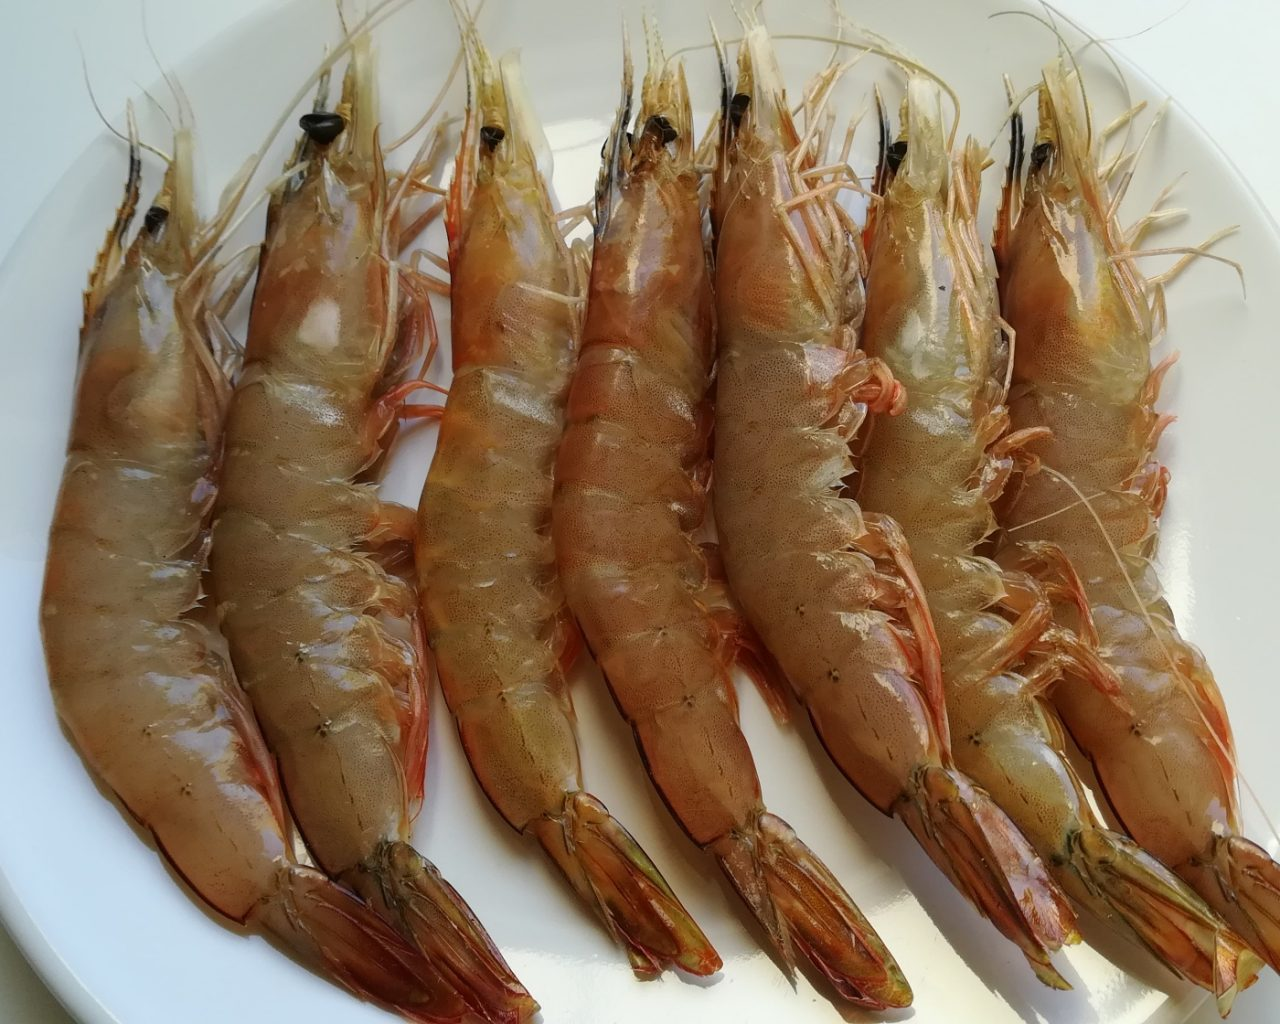
\includegraphics[scale=0.15]{crevettes.jpg}
            }
            \only<4>{
              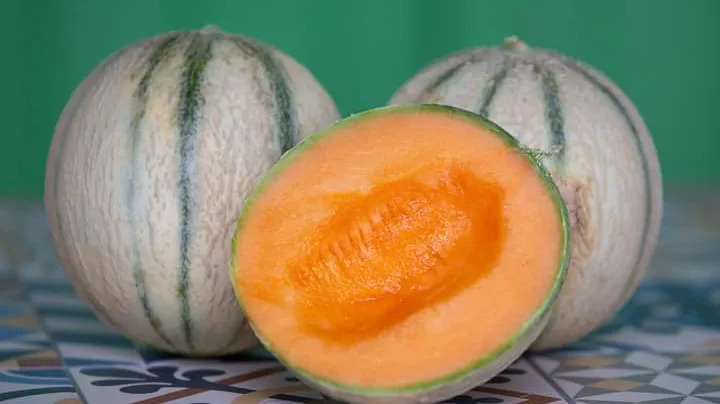
\includegraphics[scale=0.28]{melons.jpg}
            }
            \only<5>{
              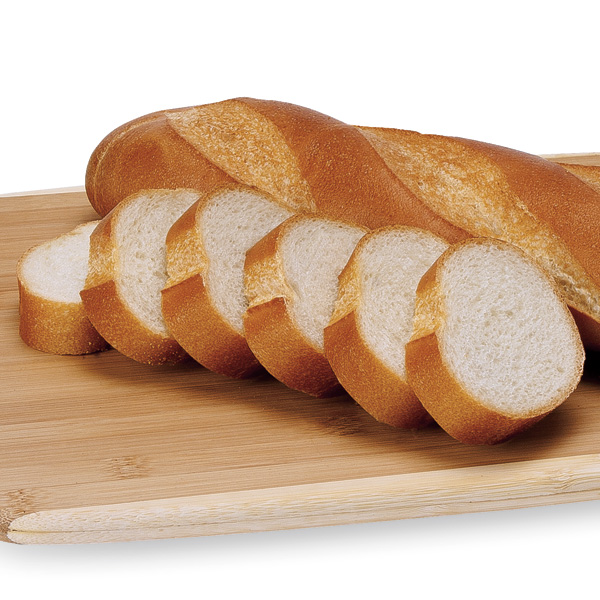
\includegraphics{tranches.jpg}
            }
            \only<6>{
              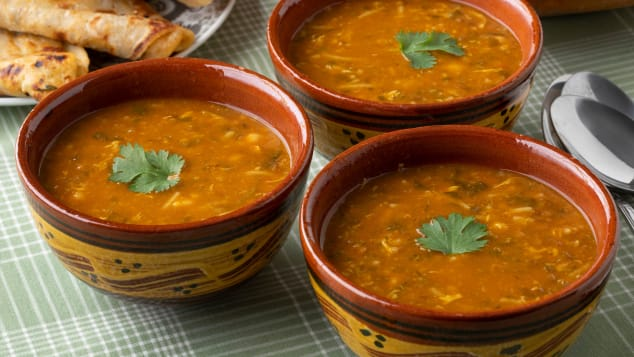
\includegraphics[scale=0.33]{bols.jpg}
            }
            \only<7>{
              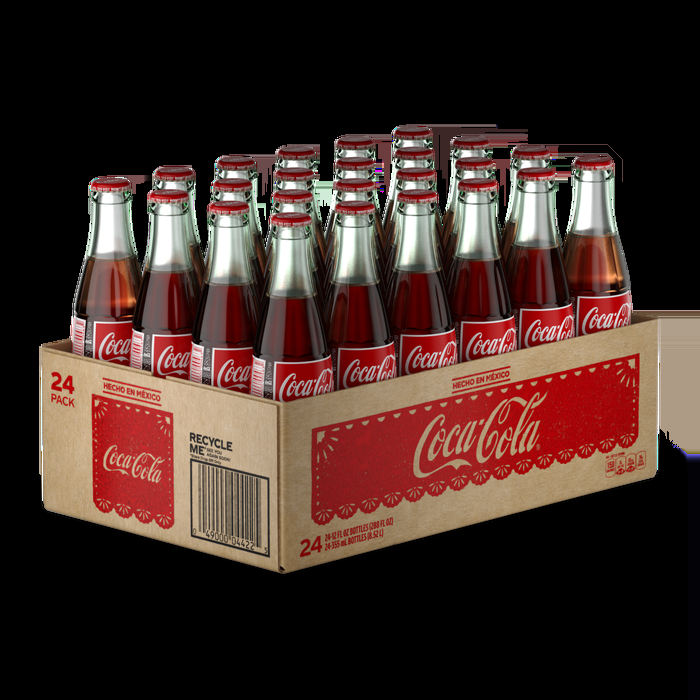
\includegraphics[scale=0.28]{bouteilles.jpg}
            }
          \end{center}
        \end{minipage}
    \end{columns}
  \end{frame}

  \begin{frame}{}
    \begin{center}
      \Large Quiz
    \end{center}
  \end{frame}

  \begin{frame}{Qu'est-ce qu'il a acheté?}
    Avec un/e partenaire, imaginez tout ce que Philippe aurait pu acheter.
    Ensuite, écris un aliment pour chaque numéro sur le tableau. \\
    \tinygloss{With a partner, imagine all the things that Philippe might have bought.
    Then, write one food for each number on the board.}
    \begin{description}
      \item[] \textbf{Modèle:} \emph{Il en a acheté une douzaine.}
      \item[E1:] Il a acheté une douzaine d'œufs.
      \item[E2:] Il a acheté une douzaine de citrons.
    \end{description}
    \begin{columns}
      \column{0.5\textwidth}
        \begin{enumerate}
          \item Il en a pris un pot.
          \item Il en a acheté un morceau.
          \item Il en a pris une douzaine.
          \item Il en a acheté une bouteille.
        \end{enumerate}
        \column{0.5\textwidth}
        \begin{enumerate}
          \setcounter{enumi}{4}
          \item Il en a pris deux paquets.
          \item Il en a acheté un kilo.
          \item Il en a demandé dix tranches.
          \item Il en a acheté une boîte.
        \end{enumerate}
    \end{columns}
  \end{frame}

  \begin{frame}{Tu en as combien?}
    Avec un/e partenaire, dis-lui combien tu as pour chaque numéro en utilisant le pronom \lexi{en}. \\
    \tinygloss{With a partner, tell them how many you have for each number using the pronoun \lexi{en}.}
    \begin{description}
      \item[] \textbf{Modèle:} \emph{des sœurs}
      \item[E1:] J'en ai deux. Elles s'appellent Holly et Amy.
      \item[E2:] Je n'en ai pas.
    \end{description}
    \begin{columns}
      \column{0.5\textwidth}
        \begin{enumerate}
          \item des sœurs
          \item des frères
          \item des amis
          \item des problèmes
        \end{enumerate}
        \column{0.5\textwidth}
        \begin{enumerate}
          \setcounter{enumi}{4}
          \item de l'argent
          \item des devoirs
          \item des responsabilités
          \item des vacances
        \end{enumerate}
    \end{columns}
  \end{frame}

  \begin{frame}{}
    \begin{center}
      \Large Questions?
    \end{center}
  \end{frame}
\end{document}
